%%%%%%%%%%%%%%%%%%%%%%%%%%%%%%%%%%%%%%%%%%
% Engineering problems / LaTeX Template
%		Semester 5
%		Institut d'Optique Graduate School
%%%%%%%%%%%%%%%%%%%%%%%%%%%%%%%%%%%%%%%%%%
%	5N-OptoElec-Bloc1	/ caractérisation statique
%%%%%%%%%%%%%%%%%%%%%%%%%%%%%%%%%%%%%%%%%%
%
% Created by:
%	Julien VILLEMEJANE - 16/jul/2024
% Modified by: Fabienne 06/09/24
%	
%
%%%%%%%%%%%%%%%%%%%%%%%%%%%%%%%%%%%%%%%%%%
% Professional Newsletter Template
% LaTeX Template
% Version 1.0 (09/03/14)
%
% Created by:
% Bob Kerstetter (https://www.tug.org/texshowcase/) and extensively modified by:
% Vel (vel@latextemplates.com)
% 
% This template has been downloaded from:
% http://www.LaTeXTemplates.com
%
% License:
% CC BY-NC-SA 3.0 (http://creativecommons.org/licenses/by-nc-sa/3.0/)
%
%%%%%%%%%%%%%%%%%%%%%%%%%%%%%%%%%%%%%%%%%

\documentclass[a4paper,11pt]{article} % The default font size is 10pt; 11pt and 12pt are alternatives

\usepackage{opto_elec_villemejane}


%%%%%%%%%%%%%%%%%%%%%%%%%%%%%%%%%%%%%%%%%%%%%%%%
%%%%%%%%%%%%%%%%%%%%%%%%%%%%%%%%%%%%%%%%%%%%%%%%
%%%%%%%%%%%%%%%%%%%%%%%%%%%%%%%%%%%%%%%%%%%%%%%%
%%%%%%%%%%%%%%%%%%%%%%%%%%%%%%%%%%%%%%%%%%%%%%%%
\begin{document}


% Page de garde
\begin{titlepage}

\begin{center}
	\begin{minipage}{2.5cm}
	\begin{center}
		
\includegraphics[width=8cm]{images/Logo-LEnsE.png}
	\end{center}
\end{minipage}\hfill
\begin{minipage}{10cm}
	\begin{center}
	\textbf{Institut d'Optique Graduate School }\\[0.1cm]
    \textbf{TP d'Opto-Électronique}


	\end{center}
\end{minipage}\hfill


\vspace{5cm}


{\huge \bfseries \textsc{Opto-Électronique}} \\[0.5cm]
{\large \bfseries Travaux Pratiques} \\[0.2cm]
Semestre 5

\vspace{2cm}
% Title
\rule{\linewidth}{0.3mm} \\[0.4cm]
{ \huge \bfseries\color{violet_iogs} Mettre en \oe{}uvre des montages de photodétection \\[0.4cm] }
\rule{\linewidth}{0.3mm} \\[1cm]
{\huge Bloc 3}

\vfill

% Bottom of the page
%{\textbf{\large {Année universitaire} 2024-2025}}

\end{center}
\end{titlepage}

\newpage
\strut % empty page
% Liens vers ressources
\newpage
\pagestyle{empty}

\begin{minipage}[c]{.25\linewidth}
	
\includegraphics[width=5cm]{images/Logo-LEnsE.png}
\end{minipage} \hfill
\begin{minipage}[c]{.4\linewidth}

\begin{center}
\vspace{0.3cm}
{\Large \textsc{Opto-Électronique}}

\medskip

5N-027-SCI \qquad \textbf{\Large TP Bloc 3}

\end{center}
\end{minipage}\hfill

\vspace{0.5cm}

\noindent \rule{\linewidth}{1pt}

{\noindent\Large \rule[-7pt]{0pt}{30pt} \textbf{Mise en \oe{}uvre de montages de photodétection}}

\noindent \rule{\linewidth}{1pt}

{\large A l'issue des séances de TP et de TD concernant le bloc 3, les étudiant$\cdot$es seront capables de \textbf{mettre en oeuvre des montages de
photodétection} et de comparer leurs performances fréquentielles et temporelles.

\medskip

\textit{Les sujets de TD ne sont pas inclus dans ce document.}

\medskip

\textit{Ce sujet est disponible au format électronique sur le site du LEnsE - https://lense.institutoptique.fr/ dans la rubrique Année / Première Année / Opto-Electronique S5 / Bloc 3.}

\noindent \rule{\linewidth}{1pt}

\medskip

Pour cela, ils$\cdot$elles %[FaB]devront être
seront capables de~:

\begin{itemize}
	\item Réaliser un circuit d'émission
	\item Caractériser un montage de photodétection (simple, suiveur, transimpédance, transimpédance avec filtrage)
	\item Choisir et adapter les éléments d'un montage de photodétection en fonction d'une application donnée
\end{itemize}


\noindent \rule{\linewidth}{1pt}

\medskip

\textbf{\large Liste des missions}

\begin{description}
	\item[Mission 3.1] \hyperref[mission31]{Réaliser un circuit d'émission à LED}
	\item[Mission 3.2] \hyperref[mission32]{Mettre en oeuvre et caractériser un circuit de photodétection simple}
	\item[Mission 3.3] \hyperref[mission33]{Mettre en oeuvre et caractériser un circuit de photodétection incluant un montage suiveur}
	\item[Mission 3.4] \hyperref[mission34]{Mettre en oeuvre et caractériser un circuit de photodétection de type transimpédance}
	\item[Mission 3.5] \hyperref[mission35]{Mettre en oeuvre et caractériser un circuit de photodétection de type transimpédance amélioré}
	\item[Mission 3.6] Choisir et adapter un montage de photodétection à une application donnée
\end{description}

\noindent \rule{\linewidth}{1pt}

\medskip

\textbf{\large Liste des autres ressources}
\begin{itemize}
	\item \hyperref[ressource:ModeleTrans]{Montage transimpédance : modélisation}
	\item \hyperref[fiche:Led]{Fiche : Diode / LED / Photodiode}
	\item \hyperref[fiche:Photodetect]{Fiche : Photodétection}
	\item \hyperref[fiche:AnHaOrdre2]{Fiche : Analyse Harmonique / Ordre 2}
\end{itemize}



\newpage
\strut % empty page

% Missions
%[FaB]\newpage
\pagestyle{empty}

\begin{minipage}[c]{.25\linewidth}
	
\includegraphics[width=4cm]{images/Logo-LEnsE.png}
\end{minipage} \hfill
\begin{minipage}[c]{.4\linewidth}

\begin{center}
\vspace{0.3cm}
{\Large \textsc{Opto-Electronique}}

\medskip

5N-027-SCI \qquad \textbf{\Large TP Bloc 3}

\end{center}
\end{minipage}\hfill

\vspace{0.5cm}

\noindent \rule{\linewidth}{1pt}

{\noindent\Large \textbf{Mission 3.1} / Réaliser un circuit d'émission à LED} 

\vspace{-0.5cm}

\begin{center}
\noindent \rule{\linewidth}{1pt}

Durée conseillée : 60 min / Séance 3 ou 4

\vspace{-0.2cm}
\noindent \rule{\linewidth}{1pt}
\end{center}

%%%%%%%%%%%%%%%%%%%%%%%%%%%%%%%%%%
\section{Objectif de la mission}
\label{mission31}

On se propose de \textbf{réaliser un circuit d'émission} d'un flux lumineux pour \textbf{transmettre un signal sinusoïdal} et de valider son fonctionnement.

%%%%%%%%%%%%%%%%%%%%%%%%%%%%%%%%%%
%%%%%%%%%%%%%%%%%%%%%%%%%%%%%%%%%%
%%%%%%%%%%%%%%%%%%%%%%%%%%%%%%%%%%
\section{Ressources}

Vous pouvez utiliser la fiche résumée suivante : 

\begin{itemize}
	\item \hyperref[fiche:Led]{Fiche : Diode / LED / Photodiode}
\end{itemize}


\subsection{LED Rouge}

On utilisera une LED rouge de type \textbf{Kingbrigth L-1503ID} ($V_f = 2\operatorname{V}$, $I_{fmax} = 25~mA$).

\subsection{Mise en oeuvre}

\Quest Proposer un montage permettant de faire fonctionner la LED dans sa zone d'émission. Comment choisir la résistance de protection de la LED ? 

\Quest Quelle forme de tension appliquée ? Comment régler les différents appareils de mesure pour éviter de dégrader la LED et garantir un flux lumineux sinusoïdal ?

\Manip Réaliser le montage.

\Quest Proposer une méthode pour valider le bon fonctionnement de votre montage (sans utiliser de système basé sur la mesure du flux lumineux...).

\Manip Valider le fonctionnement du montage.

%%%%%%%%%%%%%%%%%%%%%%%%%%%%%%%%%%
%%%%%%%%%%%%%%%%%%%%%%%%%%%%%%%%%%
\section{Livrables}


Une \textbf{fiche de manipulation} en ligne (partagée dans le cahier de laboratoire) rappelant :

\begin{itemize}
	\item les choix technologiques réalisés (schémas de câblage et valeur des composants)
	\item le choix des réglages des instruments (schémas de mesure)
	\item les courbes obtenues
\end{itemize}

Une \textbf{analyse} du résultat obtenu.


%%%%%%%%%%%%%%%%%%%%%%%%%%%%%%%%%%
%%%%%%%%%%%%%%%%%%%%%%%%%%%%%%%%%%
%[FaB]\newpage
\pagestyle{empty}

\begin{minipage}[c]{.25\linewidth}
	
\includegraphics[width=4cm]{images/Logo-LEnsE.png}
\end{minipage} \hfill
\begin{minipage}[c]{.4\linewidth}

\begin{center}
\vspace{0.3cm}
{\Large \textsc{Opto-Electronique}}

\medskip

5N-027-SCI \qquad \textbf{\Large TP Bloc 3}

\end{center}
\end{minipage}\hfill

\vspace{0.5cm}

\noindent \rule{\linewidth}{1pt}

{\noindent\Large \textbf{Mission 3.2} / Mettre en \oe{}uvre et caractériser un circuit de photodétection simple} 

\vspace{-0.5cm}

\begin{center}
\noindent \rule{\linewidth}{1pt}

Durée conseillée : 90 min / Séance 3 ou 4

\vspace{-0.2cm}
\noindent \rule{\linewidth}{1pt}
\end{center}

%%%%%%%%%%%%%%%%%%%%%%%%%%%%%%%%%%
\section{Objectif de la mission}
\label{mission32}

On se propose de \textbf{réaliser un circuit de photodétection "simple"} et de \textbf{caractériser ses performances dynamiques} (réponse en fréquence notamment).

%%%%%%%%%%%%%%%%%%%%%%%%%%%%%%%%%%
%%%%%%%%%%%%%%%%%%%%%%%%%%%%%%%%%%
%%%%%%%%%%%%%%%%%%%%%%%%%%%%%%%%%%
\section{Ressources}

\begin{itemize}
	\item \hyperref[fiche:Photodetect]{Fiche : Photodétection}
\end{itemize}


\subsection{Circuit à étudier}

\begin{multicols}{2}
On se propose d'analyser le circuit ci-contre, avec $R_{PHD} = 100\operatorname{k\Omega}$.


\Quest Quel est le lien entre $V_S$ et $I_{photo}$ ? Puis entre $I_{photo}$ et le flux lumineux capté par la photodiode $\Phi_e$ ?

\Quest Si le flux lumineux reçu est sinusoïdal, quelle sera la forme de la tension de sortie $V_S$ ? Quelles sont les limites en amplitude de ce montage ?

\Manip Réaliser le montage. Placer-le devant le montage d'émission réalisé dans la mission 3.1.

\medskip

\columnbreak

\begin{center}
\begin{circuitikz}
	\draw (0,0) to[battery2, invert] (0,4.5) -- (2,4.5);
	% fleche
	\draw (-0.5,0.3) edge[->] (-0.5,4.2);
	\node (Ein) at (-1,2.25){$E$};
	
	\draw (2,2) to[empty photodiode, *-*] (2,4.5) to[short, -o] ++(1.5,0);
	\draw (2,2.8) to[short, i = $I_{photo}$, current arrow scale=8] ++(0,-0.5);

	\draw (2,2) to[R=$R_{PHD}$, *-*] (2,0) -- (0,0);
	\draw (2,2) to[short, -o] ++(1.5,0);
	\draw (1,0) node[ground](GND){};
	\draw (2,0) to[short, -o] ++(1.5,0);
	% fleche
	\draw (3.5,2.3) edge[->] (3.5,4.2); \node (Ud) at (4,3.25){$u_d$};
	% fleche
	\draw (3.5,0.3) edge[->, green!40!black] (3.5,1.7); \node[text=green!40!black] (US) at (4,1){$V_S$};
	\draw (3.5,0) to[short, -o] ++(0,0);
\end{circuitikz}
\end{center}

\end{multicols}

\Manip Relever les formes du courant $I_f$ dans la LED et de la tension $V_S$ pour diverses valeurs de fréquence du signal d'entrée.

\Quest Quel est l'impact de $E$ sur la tension de sortie $V_S$ ?

\Quest Quelle est la forme théorique de la réponse en fréquence de ce montage ?




\subsection{Réponse en fréquence}

\Manip Tracer l'allure rapide de la réponse en fréquence en gain de ce système pour des fréquences allant de $100~\operatorname{Hz}$ à $1~\operatorname{MHz}$.

\Manip Faire une mesure de la bande-passante du montage.

\Manip Reproduire les deux précédentes étapes pour des valeurs $R_{PHD} = 10\operatorname{k\Omega}$ et $R_{PHD} = 1\operatorname{M\Omega}$. 

\Quest Quel est alors l'impact de $R_{PHD}$ sur les performances du montage ?

\subsection{Réponse indicielle}

\Manip Tracer la réponse indicielle de ce système pour les 3 valeurs de résistance proposées précédemment : $R_{PHD} = 10\operatorname{k\Omega}$, $R_{PHD} = 100\operatorname{k\Omega}$ et $R_{PHD} = 1\operatorname{M\Omega}$.

\Manip Mesurer le temps de réponse à 95\% dans chacun des cas.

\Quest Comparer les résultats obtenus avec les mesures de bande-passante.

%%%%%%%%%%%%%%%%%%%%%%%%%%%%%%%%%%
%%%%%%%%%%%%%%%%%%%%%%%%%%%%%%%%%%
\section{Modélisation}

Afin d'expliquer le phénomène observé précédemment, il est possible d'affiner le modèle utilisé pour l'étude du montage précédent en prenant en compte les éléments "perturbateurs".

Voici le modèle plus complet du montage étudié précédemment.

\begin{center}
\begin{circuitikz}
	% blocs
	\fill[green,fill opacity=.1] (-0.4,-0.2) rectangle (0.5,5.2);
	\fill[blue,fill opacity=.1] (4.8,2.2) rectangle (10.6,-0.2);	
	\fill[orange,fill opacity=.1] (1.5,5.2) rectangle (5.1,2.3);
	% legende blocs
	%\fill[green,fill opacity=.1] (9,5.5) rectangle (11,4.7);
	%\node (pol) at (10,5.1){Polarisation};
	%\fill[orange,fill opacity=.1] (9,4.5) rectangle (11,3.7);
	%\node (pol) at (10,4.1){Photodiode};	
	%\fill[blue,fill opacity=.1] (9,3.5) rectangle (11,2.7);
	%\node (pol) at (10,3.1){Affichage};	
	% circuit
	\draw (-0.5,0.3) edge[->] (-0.5,4.7); \node (Ein) at (-1,2.5){$E$};
	\draw (0,0) to[battery2, invert] (0,5) -- (2,5) to[I, *-*] (2,2.5) -- (2,2) to[R=$R_{PHD}$, *-*] (2,0) -- (0,0);
	\draw (2,3.3) to[short, i = $ I_{photo}$, current arrow scale=10] ++(0,-0.5);
	\draw (2,5) -- (3.5,5) to[C=$C_{PHD}$] (3.5,2.5) -- (2,2.5);
	\draw (1.3,2.8) edge[->] (1.3,4.7); 	\node (Ud) at (0.7,3.5){$u_d$};
		
	\draw (3.5,0.3) edge[->, green!40!black] (3.5,1.7); \node[text=green!40!black] (US) at (4,1){$V_S$};
	
	\draw (2,2) -- (5.5,2) to[C=$C_{cab}$, *-*] (5.5,0) -- (2,0);
	\draw (5.5,2) -- (7.5,2) to[C=$C_{osc}$, *-*] (7.5,0) -- (5.5,0);
	\draw (7.5,2) -- (9.5,2) to[R=$R_{osc}$] (9.5,0) -- (7.5,0);

\end{circuitikz}
\end{center}


\Quest A quoi correspondent les différents éléments présents ?

\Quest A partir des mesures réalisées précédemment, comment remonter aux valeurs du modèle précédent ? Donner les valeurs des différents éléments qu'il est possible de calculer.

%%%%%%%%%%%%%%%%%%%%%%%%%%%%%%%%%%
%%%%%%%%%%%%%%%%%%%%%%%%%%%%%%%%%%
\section{Livrables}


Une \textbf{fiche de manipulation} en ligne (partagée dans le cahier de laboratoire) rappelant :

\begin{itemize}
	\item les protocoles de mesure et de réglage (schémas de mesure, de câblage)
	\item les tableaux de mesures et les courbes obtenues
\end{itemize}

Une \textbf{analyse} du résultat obtenu, en particulier le lien entre le gain, la bande-passante du montage, le temps de réponse et la valeur de $R_{PHD}$.

Un \textbf{tableau comparatif} de ces différents éléments pour les 3 valeurs de $R_{PHD}$.

%%%%%%%%%%%%%%%%%%%%%%%%%%%%%%%%%%
%%%%%%%%%%%%%%%%%%%%%%%%%%%%%%%%%%
%[FaB]\newpage
\pagestyle{empty}

\begin{minipage}[c]{.25\linewidth}
	
\includegraphics[width=4cm]{images/Logo-LEnsE.png}
\end{minipage} \hfill
\begin{minipage}[c]{.4\linewidth}

\begin{center}
\vspace{0.3cm}
{\Large \textsc{Opto-Electronique}}

\medskip

5N-027-SCI \qquad \textbf{\Large TP Bloc 3}

\end{center}
\end{minipage}\hfill

\vspace{0.5cm}

\noindent \rule{\linewidth}{1pt}

{\noindent\Large \textbf{Mission 3.3} / Mettre en \oe{}uvre et caractériser un circuit de photodétection incluant un montage suiveur} 

\vspace{-0.5cm}

\begin{center}
\noindent \rule{\linewidth}{1pt}

Durée conseillée : 60 min / Séance 5

\vspace{-0.2cm}
\noindent \rule{\linewidth}{1pt}
\end{center}

%%%%%%%%%%%%%%%%%%%%%%%%%%%%%%%%%%
\section{Objectif de la mission}
\label{mission33}

On se propose d'\textbf{améliorer les performances dynamiques} du montage précédent en ajoutant un \textbf{montage suiveur} (basé sur un amplificateur linéaire intégré) entre le montage simple et les éléments de mesure (oscilloscope).

On souhaite également \textbf{vérifier les performances dynamiques} (réponse en fréquence notamment) de ce nouveau montage et conclure sur l'intérêt de l'ajout d'un étage suiveur.

%%%%%%%%%%%%%%%%%%%%%%%%%%%%%%%%%%
%%%%%%%%%%%%%%%%%%%%%%%%%%%%%%%%%%
%%%%%%%%%%%%%%%%%%%%%%%%%%%%%%%%%%
\section{Ressources}

Vous pouvez utiliser les fiches résumées suivantes : 

\begin{itemize}	
	\item \href{https://lense.institutoptique.fr/ressources/Annee1/Electronique/fiches/2020_FR_Photodetection.pdf}{Photodétection}
	\item \href{https://lense.institutoptique.fr/ressources/Annee1/Electronique/fiches/2021_FR_ALI.pdf}{Amplificateur Linéaire Intégré}
	\item \href{https://lense.institutoptique.fr/ressources/Annee1/Electronique/fiches/2020_FR_FiltreOrdre1.pdf}{Filtrage du premier ordre}
\end{itemize}

\subsection{Circuit à étudier}

On se propose d'analyser le circuit ci-dessous, avec $R_{PHD} = 100\operatorname{k\Omega}$. L'amplificateur linéaire intégré sera alimenté à l'aide d'une alimentation symétrique +10V / -10V.

\medskip

\begin{center}
\begin{circuitikz}
	\draw (0,0) to[battery2, invert] (0,4.5) -- (2,4.5);
	% fleche
	\draw (-0.5,0.3) edge[->] (-0.5,4.2);
	\node (Ein) at (-1,2.25){$E$};
	
	\draw (2,2) to[empty photodiode] (2,4.5);
	\draw (2,2.8) to[short, i = $I_{photo}$, current arrow scale=8] ++(0,-0.5);

	\draw (2,2) to[R=$R_{PHD}$, *-*] (2,0) -- (0,0);
	\draw (2,2) -- ++(2.5,0);
	\draw (1,0) node[ground](GND){};
	\draw (2,0) to[short, -o] ++(1.5,0) coordinate(VRG);
	% fleche
	\draw (3.5,0.3) edge[->, green!40!black] (3.5,1.7); \node[text=green!40!black] (UR) at (4.3,1){$V_{RPHD}$};
	\draw (3.5,0) to[short, -o] ++(0,0);
	
	\draw (4.5,2) node[op amp, fill=blue!10!white, anchor=+](A1) {\texttt{ALI1}};
	\draw (A1.-) to[short] ++(-.5,0) coordinate(A) to[short] ++(0,1.5) coordinate(B) to[short] (B -| A1.out) to[short, -*] (A1.out);
	\draw (A1.+) to[short,-o] ++(-1,0) coordinate(C);
	\draw (A1.out) to[short,-o] ++(1,0) coordinate(D);	
	\draw (VRG) -- (VRG -| A1.out) coordinate(VOUTGND);
	\draw (VOUTGND) to[short,-o] ++(1,0) coordinate(VSGND);
	
	% fleche
	\draw (VSGND) ++(0,0.3) edge[->, green!40!black] ($ (D) - (0,0.3) $); \node[text=green!40!black] (US) at ($ (VSGND)!.5!(D) + (0.5,0) $){$V_S$};	% point central entre les deux points
\end{circuitikz}
\end{center}

\Quest Quel est le lien entre $V_S$ et $V_{RPHD}$ ? Puis entre $V_S$ et $I_{photo}$ ? Puis entre $I_{photo}$ et le flux lumineux capté par la photodiode $\Phi_e$ ?

\Quest Quelle est la forme théorique de la réponse en fréquence de ce montage ?

\subsection{Réponse en fréquence}

\Manip Tracer l'allure rapide de la réponse en fréquence en gain de ce système pour des fréquences allant de $100~\operatorname{Hz}$ à $1~\operatorname{MHz}$.

\Manip Faire une mesure de la bande-passante du montage.

\Manip Reproduire les deux précédentes étapes pour des valeurs $R_{PHD} = 10\operatorname{k\Omega}$ et $R_{PHD} = 1\operatorname{M\Omega}$. 

\Quest Quel est alors l'impact de $R_{PHD}$ sur le montage ?

\Quest Quel est l'apport du montage suiveur ?

%%%%%%%%%%%%%%%%%%%%%%%%%%%%%%%%%%
%%%%%%%%%%%%%%%%%%%%%%%%%%%%%%%%%%
\section{Livrables}

Une \textbf{fiche de manipulation} en ligne (partagée dans le cahier de laboratoire) rappelant :

\begin{itemize}
	\item les protocoles de mesure et de réglage (schémas de mesure, de câblage)
	\item les tableaux de mesures et les courbes obtenues
\end{itemize}

Une \textbf{analyse} du résultat obtenu, en particulier le lien entre le gain, la bande-passante du montage, le temps de réponse et la valeur de $R_{PHD}$.

Une \textbf{analyse comparative} du montage de photodétection simple (mission 3.2) et d'un montage suiveur (mission 3.3), précisant l'intérêt d'utiliser un tel montage.


%%%%%%%%%%%%%%%%%%%%%%%%%%%%%%%%%%
%%%%%%%%%%%%%%%%%%%%%%%%%%%%%%%%%%
%[FaB]\newpage
\pagestyle{empty}

\begin{minipage}[c]{.25\linewidth}
	
\includegraphics[width=4cm]{images/Logo-LEnsE.png}
\end{minipage} \hfill
\begin{minipage}[c]{.4\linewidth}

\begin{center}
\vspace{0.3cm}
{\Large \textsc{Opto-Electronique}}

\medskip

5N-027-SCI \qquad \textbf{\Large TP Bloc 3}

\end{center}
\end{minipage}\hfill

\vspace{0.5cm}

\noindent \rule{\linewidth}{1pt}

{\noindent\Large \textbf{Mission 3.4} / Mettre en \oe{}uvre et caractériser un circuit de photodétection de type transimpédance} 

\vspace{-0.5cm}

\begin{center}
\noindent \rule{\linewidth}{1pt}

Durée conseillée : 90 min / Séance 5

\vspace{-0.2cm}
\noindent \rule{\linewidth}{1pt}
\end{center}

%%%%%%%%%%%%%%%%%%%%%%%%%%%%%%%%%%
\section{Objectif de la mission}
\label{mission34}

On se propose d'\textbf{étudier le montage transimpédance}, un circuit très fréquemment utilisé pour la photodétection pour ses performances dynamiques. Ce montage est basé sur un amplificateur linéaire intégré également et permet d'augmenter la bande-passante des montages vus précédemment.

On souhaite donc \textbf{vérifier les performances dynamiques} (réponse en fréquence notamment) de ce nouveau montage et conclure sur son intérêt.

\medskip

\textit{Afin de faciliter la compréhension des phénomènes mis en jeu dans ce montage, vous pouvez vous reporter à la ressource : \hyperref[ressource:ModeleTrans]{Montage transimpédance : modélisation}.}


%%%%%%%%%%%%%%%%%%%%%%%%%%%%%%%%%%
%%%%%%%%%%%%%%%%%%%%%%%%%%%%%%%%%%
%%%%%%%%%%%%%%%%%%%%%%%%%%%%%%%%%%
\section{Ressources}

Vous pouvez utiliser les fiches résumées suivantes : 

\begin{itemize}	
	\item \href{https://lense.institutoptique.fr/ressources/Annee1/Electronique/fiches/2020_FR_Photodetection.pdf}{Photodétection}
	\item \href{https://lense.institutoptique.fr/ressources/Annee1/Electronique/fiches/2021_FR_ALI.pdf}{Amplificateur Linéaire Intégré}
\end{itemize}



\subsection{Circuit à étudier}

On se propose d'analyser le circuit ci-dessous, avec $R_{PHD} = 100\operatorname{k\Omega}$. L'amplificateur linéaire intégré sera alimenté à l'aide d'une alimentation symétrique +10V / -10V.

\begin{center}
\begin{circuitikz} 
	\node [op amp, fill=blue!10!white](A1) at (0,0){\texttt{ALI1}};
	\draw (A1.-) to[short] ++(-.5,0) coordinate(A) to[short] ++(0,1.5) coordinate(B) to[R=$R_{PHD}$] (B -| A1.out) to[short, -*] (A1.out);
	\draw (A1.-) to[short,-*] ++(-.5,0) coordinate(AA) -- ++(-1,0) coordinate(AAA) to[empty photodiode] ++(-2,0) coordinate(BB);	
	
	\draw (AAA) to[short, i = $I_{photo}$, current arrow scale=8] ++(0.5,0);
	\draw (A1.+) to[short, -*] ++(0,-1.5) coordinate(GG) node[ground]{};
	
	\draw (A1.out) to[short,-o] ++(1,0) coordinate(D);
	
	% Ground
	\draw (GG) to[short, -o] (GG -| D);
	
	\draw (BB) to[battery2] (GG -| BB) -- (GG);
	% fleche EP
	\draw ($ (GG -| BB) + (-0.8,0.3) $) edge[->, green!40!black] ($ (BB) - (0.8,0.3) $); 
	\node[text=green!40!black] (US) at ($ (GG -| BB)!.5!(BB) - (1.5,0) $){$E_P$};
	
	% fleche VS
	\draw ($ (GG -| D) + (0,0.3) $) edge[->, green!40!black] ($ (D) - (0,0.3) $); 
	\node[text=green!40!black] (US) at ($ (GG -| D)!.5!(D) - (0.5,0) $){$V_S$};	
\end{circuitikz}
\end{center}

\Quest Quel est le lien entre $V_S$ et $I_{photo}$ ? Puis entre $I_{photo}$ et le flux lumineux capté par la photodiode $\Phi_e$ ?

\subsection{Réponse en fréquence}

\Manip Tracer l'allure rapide de la réponse en fréquence en gain de ce système pour des fréquences allant de $100~\operatorname{Hz}$ à $1~\operatorname{MHz}$.

\Manip Faire une mesure de la bande-passante du montage.

\Manip Reproduire les deux précédentes étapes pour des valeurs $R_{PHD} = 10\operatorname{k\Omega}$ et $R_{PHD} = 1\operatorname{M\Omega}$. 

\Quest Quel est alors l'impact de $R_{PHD}$ sur le montage ?

\subsection{Réponse indicielle}

\Manip Tracer la réponse indicielle de ce système pour les 3 valeurs de résistance proposées précédemment : $R_{PHD} = 10\operatorname{k\Omega}$, $R_{PHD} = 100\operatorname{k\Omega}$ et $R_{PHD} = 1\operatorname{M\Omega}$.

\Manip Mesurer le temps de réponse à 95\% dans chacun des cas.

\Quest Comparer les résultats obtenus avec les mesures de bande-passante.


%%%%%%%%%%%%%%%%%%%%%%%%%%%%%%%%%%
%%%%%%%%%%%%%%%%%%%%%%%%%%%%%%%%%%
\section{Livrables}

Une \textbf{fiche de manipulation} en ligne (partagée dans le cahier de laboratoire) rappelant :

\begin{itemize}
	\item les protocoles de mesure et de réglage (schémas de mesure, de câblage)
	\item les tableaux de mesures et les courbes obtenues
\end{itemize}

Une \textbf{analyse} du résultat obtenu, en particulier le lien entre le gain, la bande-passante du montage, le temps de réponse et la valeur de $R_{PHD}$.

Une \textbf{analyse comparative} des montages de photodétection simple (mission 3.2), avec un montage suiveur (mission 3.3) et transimpédance (mission 3.4), précisant l'intérêt d'utiliser un tel montage.



%%%%%%%%%%%%%%%%%%%%%%%%%%%%%%%%%%
%%%%%%%%%%%%%%%%%%%%%%%%%%%%%%%%%%
%[FaB]\newpage
\pagestyle{empty}

\begin{minipage}[c]{.25\linewidth}
	
\includegraphics[width=4cm]{images/Logo-LEnsE.png}
\end{minipage} \hfill
\begin{minipage}[c]{.4\linewidth}

\begin{center}
\vspace{0.3cm}
{\Large \textsc{Opto-Electronique}}

\medskip

5N-027-SCI \qquad \textbf{\Large TP Bloc 3}

\end{center}
\end{minipage}\hfill

\vspace{0.5cm}

\noindent \rule{\linewidth}{1pt}

{\noindent\Large \textbf{Mission 3.5} / Mettre en \oe{}uvre et caractériser un circuit de photodétection de type transimpédance amélioré} 

\vspace{-0.5cm}

\begin{center}
\noindent \rule{\linewidth}{1pt}

Durée conseillée : 60 min / Séance 5

\vspace{-0.2cm}
\noindent \rule{\linewidth}{1pt}
\end{center}

%%%%%%%%%%%%%%%%%%%%%%%%%%%%%%%%%%
\section{Objectif de la mission}
\label{mission35}

On se propose de \textbf{s'affranchir d'un des défauts majeur du montage transimpédance}. On souhaite donc \textbf{vérifier les performances dynamiques} (réponse en fréquence notamment) de ce nouveau montage et conclure sur son intérêt.

\medskip

\textit{Afin de faciliter la compréhension des phénomènes mis en jeu dans ce montage, vous pouvez vous reporter à la ressource : \hyperref[ressource:ModeleTrans]{Montage transimpédance : modélisation}.}

%%%%%%%%%%%%%%%%%%%%%%%%%%%%%%%%%%
%%%%%%%%%%%%%%%%%%%%%%%%%%%%%%%%%%
%%%%%%%%%%%%%%%%%%%%%%%%%%%%%%%%%%
\section{Ressources}

Vous pouvez utiliser les fiches résumées suivantes : 

\begin{itemize}	
	\item \href{https://lense.institutoptique.fr/ressources/Annee1/Electronique/fiches/2020_FR_Photodetection.pdf}{Photodétection}
	\item \href{https://lense.institutoptique.fr/ressources/Annee1/Electronique/fiches/2021_FR_ALI.pdf}{Amplificateur Linéaire Intégré}
\end{itemize}


\subsection{Circuit à étudier}

On se propose d'analyser le circuit ci-dessous, avec $R_{PHD} = 100\operatorname{k\Omega}$. L'amplificateur linéaire intégré sera alimenté à l'aide d'une alimentation symétrique +10V / -10V.

\begin{center}
\begin{circuitikz} 
	\node [op amp, fill=blue!10!white](A1) at (0,0){\texttt{ALI1}};
	\draw (A1.-) to[short] ++(-.5,0) coordinate(A) to[short, -*] ++(0,1.5) coordinate(B) to[R=$R_{PHD}$] (B -| A1.out) to[short, -*] (A1.out);
	\draw (B) -- ++(0,1.5) coordinate(B2) to[C=$C_{T}$] (B2 -| A1.out) to[short,-*] (B -| A1.out);
	\draw (A1.-) to[short,-*] ++(-.5,0) coordinate(AA) -- ++(-1,0) coordinate(AAA) to[empty photodiode] ++(-2,0) coordinate(BB);	
	
	\draw (AAA) to[short, i = $I_{photo}$, current arrow scale=8] ++(0.5,0);
	\draw (A1.+) to[short, -*] ++(0,-1.5) coordinate(GG) node[ground]{};
	
	\draw (A1.out) to[short,-o] ++(1,0) coordinate(D);
	
	% Ground
	\draw (GG) to[short, -o] (GG -| D);
	
	\draw (BB) to[battery2] (GG -| BB) -- (GG);
	% fleche EP
	\draw ($ (GG -| BB) + (-0.8,0.3) $) edge[->, green!40!black] ($ (BB) - (0.8,0.3) $); 
	\node[text=green!40!black] (US) at ($ (GG -| BB)!.5!(BB) - (1.5,0) $){$E_P$};
	
	% fleche VS
	\draw ($ (GG -| D) + (0,0.3) $) edge[->, green!40!black] ($ (D) - (0,0.3) $); 
	\node[text=green!40!black] (US) at ($ (GG -| D)!.5!(D) - (0.5,0) $){$V_S$};	
\end{circuitikz}
\end{center}

\Quest Quelle valeur de $C_T$ faut-il pour éliminer le phénomène de résonance ?

\subsection{Réponse en fréquence}

\Manip Tracer l'allure rapide de la réponse en fréquence en gain de ce système pour des fréquences allant de $100~\operatorname{Hz}$ à $1~\operatorname{MHz}$.

\Manip Faire une mesure de la bande-passante du montage.

\subsection{Réponse indicielle}

\Manip Tracer la réponse indicielle de ce système.


%%%%%%%%%%%%%%%%%%%%%%%%%%%%%%%%%%
%%%%%%%%%%%%%%%%%%%%%%%%%%%%%%%%%%
\section{Livrables}


Une \textbf{fiche de manipulation} en ligne (partagée dans le cahier de laboratoire) rappelant :

\begin{itemize}
	\item les protocoles de mesure et de réglage (schémas de mesure, de câblage)	
	\item les tableaux de mesures et les courbes obtenues
\end{itemize}

Une \textbf{analyse} du résultat obtenu.


%%%%%%%%%%%%%%%%%%%%%%%%%%%%%%%%%%
%%%%%%%%%%%%%%%%%%%%%%%%%%%%%%%%%%

\newpage
\pagestyle{empty}

\begin{minipage}[c]{.25\linewidth}
	
\includegraphics[width=4cm]{images/Logo-LEnsE.png}
\end{minipage} \hfill
\begin{minipage}[c]{.4\linewidth}

\begin{center}
\vspace{0.3cm}
{\Large \textsc{Opto-Electronique}}

\medskip

5N-027-SCI \qquad \textbf{\Large TP Bloc 3}

\end{center}
\end{minipage}\hfill

\vspace{0.5cm}

\noindent \rule{\linewidth}{1pt}

{\noindent\Large \textbf{Mission 3.1} / Réaliser un circuit d'émission à LED} 

\vspace{-0.5cm}

\begin{center}
\noindent \rule{\linewidth}{1pt}

Durée conseillée : 60 min / Séance 3 ou 4

\vspace{-0.2cm}
\noindent \rule{\linewidth}{1pt}
\end{center}

%%%%%%%%%%%%%%%%%%%%%%%%%%%%%%%%%%
\section{Objectif de la mission}
\label{mission31}

On se propose de \textbf{réaliser un circuit d'émission} d'un flux lumineux pour \textbf{transmettre un signal sinusoïdal} et de valider son fonctionnement.

%%%%%%%%%%%%%%%%%%%%%%%%%%%%%%%%%%
%%%%%%%%%%%%%%%%%%%%%%%%%%%%%%%%%%
%%%%%%%%%%%%%%%%%%%%%%%%%%%%%%%%%%
\section{Ressources}

Vous pouvez utiliser la fiche résumée suivante : 

\begin{itemize}
	\item \hyperref[fiche:Led]{Fiche : Diode / LED / Photodiode}
\end{itemize}


\subsection{LED Rouge}

On utilisera une LED rouge de type \textbf{Kingbrigth L-1503ID} ($V_f = 2\operatorname{V}$, $I_{fmax} = 25~mA$).

\subsection{Mise en oeuvre}

\Quest Proposer un montage permettant de faire fonctionner la LED dans sa zone d'émission. Comment choisir la résistance de protection de la LED ? 

\Quest Quelle forme de tension appliquée ? Comment régler les différents appareils de mesure pour éviter de dégrader la LED et garantir un flux lumineux sinusoïdal ?

\Manip Réaliser le montage.

\Quest Proposer une méthode pour valider le bon fonctionnement de votre montage (sans utiliser de système basé sur la mesure du flux lumineux...).

\Manip Valider le fonctionnement du montage.

%%%%%%%%%%%%%%%%%%%%%%%%%%%%%%%%%%
%%%%%%%%%%%%%%%%%%%%%%%%%%%%%%%%%%
\section{Livrables}


Une \textbf{fiche de manipulation} en ligne (partagée dans le cahier de laboratoire) rappelant :

\begin{itemize}
	\item les choix technologiques réalisés (schémas de câblage et valeur des composants)
	\item le choix des réglages des instruments (schémas de mesure)
	\item les courbes obtenues
\end{itemize}

Une \textbf{analyse} du résultat obtenu.


%%%%%%%%%%%%%%%%%%%%%%%%%%%%%%%%%%
%%%%%%%%%%%%%%%%%%%%%%%%%%%%%%%%%%

\newpage
\strut % empty page
\newpage
\pagestyle{empty}

\begin{minipage}[c]{.25\linewidth}
	
\includegraphics[width=4cm]{images/Logo-LEnsE.png}
\end{minipage} \hfill
\begin{minipage}[c]{.4\linewidth}

\begin{center}
\vspace{0.3cm}
{\Large \textsc{Opto-Electronique}}

\medskip

5N-027-SCI \qquad \textbf{\Large TP Bloc 3}

\end{center}
\end{minipage}\hfill

\vspace{0.5cm}

\noindent \rule{\linewidth}{1pt}

{\noindent\Large \textbf{Mission 3.2} / Mettre en \oe{}uvre et caractériser un circuit de photodétection simple} 

\vspace{-0.5cm}

\begin{center}
\noindent \rule{\linewidth}{1pt}

Durée conseillée : 90 min / Séance 3 ou 4

\vspace{-0.2cm}
\noindent \rule{\linewidth}{1pt}
\end{center}

%%%%%%%%%%%%%%%%%%%%%%%%%%%%%%%%%%
\section{Objectif de la mission}
\label{mission32}

On se propose de \textbf{réaliser un circuit de photodétection "simple"} et de \textbf{caractériser ses performances dynamiques} (réponse en fréquence notamment).

%%%%%%%%%%%%%%%%%%%%%%%%%%%%%%%%%%
%%%%%%%%%%%%%%%%%%%%%%%%%%%%%%%%%%
%%%%%%%%%%%%%%%%%%%%%%%%%%%%%%%%%%
\section{Ressources}

\begin{itemize}
	\item \hyperref[fiche:Photodetect]{Fiche : Photodétection}
\end{itemize}


\subsection{Circuit à étudier}

\begin{multicols}{2}
On se propose d'analyser le circuit ci-contre, avec $R_{PHD} = 100\operatorname{k\Omega}$.


\Quest Quel est le lien entre $V_S$ et $I_{photo}$ ? Puis entre $I_{photo}$ et le flux lumineux capté par la photodiode $\Phi_e$ ?

\Quest Si le flux lumineux reçu est sinusoïdal, quelle sera la forme de la tension de sortie $V_S$ ? Quelles sont les limites en amplitude de ce montage ?

\Manip Réaliser le montage. Placer-le devant le montage d'émission réalisé dans la mission 3.1.

\medskip

\columnbreak

\begin{center}
\begin{circuitikz}
	\draw (0,0) to[battery2, invert] (0,4.5) -- (2,4.5);
	% fleche
	\draw (-0.5,0.3) edge[->] (-0.5,4.2);
	\node (Ein) at (-1,2.25){$E$};
	
	\draw (2,2) to[empty photodiode, *-*] (2,4.5) to[short, -o] ++(1.5,0);
	\draw (2,2.8) to[short, i = $I_{photo}$, current arrow scale=8] ++(0,-0.5);

	\draw (2,2) to[R=$R_{PHD}$, *-*] (2,0) -- (0,0);
	\draw (2,2) to[short, -o] ++(1.5,0);
	\draw (1,0) node[ground](GND){};
	\draw (2,0) to[short, -o] ++(1.5,0);
	% fleche
	\draw (3.5,2.3) edge[->] (3.5,4.2); \node (Ud) at (4,3.25){$u_d$};
	% fleche
	\draw (3.5,0.3) edge[->, green!40!black] (3.5,1.7); \node[text=green!40!black] (US) at (4,1){$V_S$};
	\draw (3.5,0) to[short, -o] ++(0,0);
\end{circuitikz}
\end{center}

\end{multicols}

\Manip Relever les formes du courant $I_f$ dans la LED et de la tension $V_S$ pour diverses valeurs de fréquence du signal d'entrée.

\Quest Quel est l'impact de $E$ sur la tension de sortie $V_S$ ?

\Quest Quelle est la forme théorique de la réponse en fréquence de ce montage ?




\subsection{Réponse en fréquence}

\Manip Tracer l'allure rapide de la réponse en fréquence en gain de ce système pour des fréquences allant de $100~\operatorname{Hz}$ à $1~\operatorname{MHz}$.

\Manip Faire une mesure de la bande-passante du montage.

\Manip Reproduire les deux précédentes étapes pour des valeurs $R_{PHD} = 10\operatorname{k\Omega}$ et $R_{PHD} = 1\operatorname{M\Omega}$. 

\Quest Quel est alors l'impact de $R_{PHD}$ sur les performances du montage ?

\subsection{Réponse indicielle}

\Manip Tracer la réponse indicielle de ce système pour les 3 valeurs de résistance proposées précédemment : $R_{PHD} = 10\operatorname{k\Omega}$, $R_{PHD} = 100\operatorname{k\Omega}$ et $R_{PHD} = 1\operatorname{M\Omega}$.

\Manip Mesurer le temps de réponse à 95\% dans chacun des cas.

\Quest Comparer les résultats obtenus avec les mesures de bande-passante.

%%%%%%%%%%%%%%%%%%%%%%%%%%%%%%%%%%
%%%%%%%%%%%%%%%%%%%%%%%%%%%%%%%%%%
\section{Modélisation}

Afin d'expliquer le phénomène observé précédemment, il est possible d'affiner le modèle utilisé pour l'étude du montage précédent en prenant en compte les éléments "perturbateurs".

Voici le modèle plus complet du montage étudié précédemment.

\begin{center}
\begin{circuitikz}
	% blocs
	\fill[green,fill opacity=.1] (-0.4,-0.2) rectangle (0.5,5.2);
	\fill[blue,fill opacity=.1] (4.8,2.2) rectangle (10.6,-0.2);	
	\fill[orange,fill opacity=.1] (1.5,5.2) rectangle (5.1,2.3);
	% legende blocs
	%\fill[green,fill opacity=.1] (9,5.5) rectangle (11,4.7);
	%\node (pol) at (10,5.1){Polarisation};
	%\fill[orange,fill opacity=.1] (9,4.5) rectangle (11,3.7);
	%\node (pol) at (10,4.1){Photodiode};	
	%\fill[blue,fill opacity=.1] (9,3.5) rectangle (11,2.7);
	%\node (pol) at (10,3.1){Affichage};	
	% circuit
	\draw (-0.5,0.3) edge[->] (-0.5,4.7); \node (Ein) at (-1,2.5){$E$};
	\draw (0,0) to[battery2, invert] (0,5) -- (2,5) to[I, *-*] (2,2.5) -- (2,2) to[R=$R_{PHD}$, *-*] (2,0) -- (0,0);
	\draw (2,3.3) to[short, i = $ I_{photo}$, current arrow scale=10] ++(0,-0.5);
	\draw (2,5) -- (3.5,5) to[C=$C_{PHD}$] (3.5,2.5) -- (2,2.5);
	\draw (1.3,2.8) edge[->] (1.3,4.7); 	\node (Ud) at (0.7,3.5){$u_d$};
		
	\draw (3.5,0.3) edge[->, green!40!black] (3.5,1.7); \node[text=green!40!black] (US) at (4,1){$V_S$};
	
	\draw (2,2) -- (5.5,2) to[C=$C_{cab}$, *-*] (5.5,0) -- (2,0);
	\draw (5.5,2) -- (7.5,2) to[C=$C_{osc}$, *-*] (7.5,0) -- (5.5,0);
	\draw (7.5,2) -- (9.5,2) to[R=$R_{osc}$] (9.5,0) -- (7.5,0);

\end{circuitikz}
\end{center}


\Quest A quoi correspondent les différents éléments présents ?

\Quest A partir des mesures réalisées précédemment, comment remonter aux valeurs du modèle précédent ? Donner les valeurs des différents éléments qu'il est possible de calculer.

%%%%%%%%%%%%%%%%%%%%%%%%%%%%%%%%%%
%%%%%%%%%%%%%%%%%%%%%%%%%%%%%%%%%%
\section{Livrables}


Une \textbf{fiche de manipulation} en ligne (partagée dans le cahier de laboratoire) rappelant :

\begin{itemize}
	\item les protocoles de mesure et de réglage (schémas de mesure, de câblage)
	\item les tableaux de mesures et les courbes obtenues
\end{itemize}

Une \textbf{analyse} du résultat obtenu, en particulier le lien entre le gain, la bande-passante du montage, le temps de réponse et la valeur de $R_{PHD}$.

Un \textbf{tableau comparatif} de ces différents éléments pour les 3 valeurs de $R_{PHD}$.

%%%%%%%%%%%%%%%%%%%%%%%%%%%%%%%%%%
%%%%%%%%%%%%%%%%%%%%%%%%%%%%%%%%%%
\newpage
\pagestyle{empty}

\begin{minipage}[c]{.25\linewidth}
	
\includegraphics[width=4cm]{images/Logo-LEnsE.png}
\end{minipage} \hfill
\begin{minipage}[c]{.4\linewidth}

\begin{center}
\vspace{0.3cm}
{\Large \textsc{Opto-Electronique}}

\medskip

5N-027-SCI \qquad \textbf{\Large TP Bloc 3}

\end{center}
\end{minipage}\hfill

\vspace{0.5cm}

\noindent \rule{\linewidth}{1pt}

{\noindent\Large \textbf{Mission 3.3} / Mettre en \oe{}uvre et caractériser un circuit de photodétection incluant un montage suiveur} 

\vspace{-0.5cm}

\begin{center}
\noindent \rule{\linewidth}{1pt}

Durée conseillée : 60 min / Séance 5

\vspace{-0.2cm}
\noindent \rule{\linewidth}{1pt}
\end{center}

%%%%%%%%%%%%%%%%%%%%%%%%%%%%%%%%%%
\section{Objectif de la mission}
\label{mission33}

On se propose d'\textbf{améliorer les performances dynamiques} du montage précédent en ajoutant un \textbf{montage suiveur} (basé sur un amplificateur linéaire intégré) entre le montage simple et les éléments de mesure (oscilloscope).

On souhaite également \textbf{vérifier les performances dynamiques} (réponse en fréquence notamment) de ce nouveau montage et conclure sur l'intérêt de l'ajout d'un étage suiveur.

%%%%%%%%%%%%%%%%%%%%%%%%%%%%%%%%%%
%%%%%%%%%%%%%%%%%%%%%%%%%%%%%%%%%%
%%%%%%%%%%%%%%%%%%%%%%%%%%%%%%%%%%
\section{Ressources}

Vous pouvez utiliser les fiches résumées suivantes : 

\begin{itemize}	
	\item \href{https://lense.institutoptique.fr/ressources/Annee1/Electronique/fiches/2020_FR_Photodetection.pdf}{Photodétection}
	\item \href{https://lense.institutoptique.fr/ressources/Annee1/Electronique/fiches/2021_FR_ALI.pdf}{Amplificateur Linéaire Intégré}
	\item \href{https://lense.institutoptique.fr/ressources/Annee1/Electronique/fiches/2020_FR_FiltreOrdre1.pdf}{Filtrage du premier ordre}
\end{itemize}

\subsection{Circuit à étudier}

On se propose d'analyser le circuit ci-dessous, avec $R_{PHD} = 100\operatorname{k\Omega}$. L'amplificateur linéaire intégré sera alimenté à l'aide d'une alimentation symétrique +10V / -10V.

\medskip

\begin{center}
\begin{circuitikz}
	\draw (0,0) to[battery2, invert] (0,4.5) -- (2,4.5);
	% fleche
	\draw (-0.5,0.3) edge[->] (-0.5,4.2);
	\node (Ein) at (-1,2.25){$E$};
	
	\draw (2,2) to[empty photodiode] (2,4.5);
	\draw (2,2.8) to[short, i = $I_{photo}$, current arrow scale=8] ++(0,-0.5);

	\draw (2,2) to[R=$R_{PHD}$, *-*] (2,0) -- (0,0);
	\draw (2,2) -- ++(2.5,0);
	\draw (1,0) node[ground](GND){};
	\draw (2,0) to[short, -o] ++(1.5,0) coordinate(VRG);
	% fleche
	\draw (3.5,0.3) edge[->, green!40!black] (3.5,1.7); \node[text=green!40!black] (UR) at (4.3,1){$V_{RPHD}$};
	\draw (3.5,0) to[short, -o] ++(0,0);
	
	\draw (4.5,2) node[op amp, fill=blue!10!white, anchor=+](A1) {\texttt{ALI1}};
	\draw (A1.-) to[short] ++(-.5,0) coordinate(A) to[short] ++(0,1.5) coordinate(B) to[short] (B -| A1.out) to[short, -*] (A1.out);
	\draw (A1.+) to[short,-o] ++(-1,0) coordinate(C);
	\draw (A1.out) to[short,-o] ++(1,0) coordinate(D);	
	\draw (VRG) -- (VRG -| A1.out) coordinate(VOUTGND);
	\draw (VOUTGND) to[short,-o] ++(1,0) coordinate(VSGND);
	
	% fleche
	\draw (VSGND) ++(0,0.3) edge[->, green!40!black] ($ (D) - (0,0.3) $); \node[text=green!40!black] (US) at ($ (VSGND)!.5!(D) + (0.5,0) $){$V_S$};	% point central entre les deux points
\end{circuitikz}
\end{center}

\Quest Quel est le lien entre $V_S$ et $V_{RPHD}$ ? Puis entre $V_S$ et $I_{photo}$ ? Puis entre $I_{photo}$ et le flux lumineux capté par la photodiode $\Phi_e$ ?

\Quest Quelle est la forme théorique de la réponse en fréquence de ce montage ?

\subsection{Réponse en fréquence}

\Manip Tracer l'allure rapide de la réponse en fréquence en gain de ce système pour des fréquences allant de $100~\operatorname{Hz}$ à $1~\operatorname{MHz}$.

\Manip Faire une mesure de la bande-passante du montage.

\Manip Reproduire les deux précédentes étapes pour des valeurs $R_{PHD} = 10\operatorname{k\Omega}$ et $R_{PHD} = 1\operatorname{M\Omega}$. 

\Quest Quel est alors l'impact de $R_{PHD}$ sur le montage ?

\Quest Quel est l'apport du montage suiveur ?

%%%%%%%%%%%%%%%%%%%%%%%%%%%%%%%%%%
%%%%%%%%%%%%%%%%%%%%%%%%%%%%%%%%%%
\section{Livrables}

Une \textbf{fiche de manipulation} en ligne (partagée dans le cahier de laboratoire) rappelant :

\begin{itemize}
	\item les protocoles de mesure et de réglage (schémas de mesure, de câblage)
	\item les tableaux de mesures et les courbes obtenues
\end{itemize}

Une \textbf{analyse} du résultat obtenu, en particulier le lien entre le gain, la bande-passante du montage, le temps de réponse et la valeur de $R_{PHD}$.

Une \textbf{analyse comparative} du montage de photodétection simple (mission 3.2) et d'un montage suiveur (mission 3.3), précisant l'intérêt d'utiliser un tel montage.


%%%%%%%%%%%%%%%%%%%%%%%%%%%%%%%%%%
%%%%%%%%%%%%%%%%%%%%%%%%%%%%%%%%%%
\newpage
\pagestyle{empty}

\begin{minipage}[c]{.25\linewidth}
	
\includegraphics[width=4cm]{images/Logo-LEnsE.png}
\end{minipage} \hfill
\begin{minipage}[c]{.4\linewidth}

\begin{center}
\vspace{0.3cm}
{\Large \textsc{Opto-Electronique}}

\medskip

5N-027-SCI \qquad \textbf{\Large TP Bloc 3}

\end{center}
\end{minipage}\hfill

\vspace{0.5cm}

\noindent \rule{\linewidth}{1pt}

{\noindent\Large \textbf{Mission 3.4} / Mettre en \oe{}uvre et caractériser un circuit de photodétection de type transimpédance} 

\vspace{-0.5cm}

\begin{center}
\noindent \rule{\linewidth}{1pt}

Durée conseillée : 90 min / Séance 5

\vspace{-0.2cm}
\noindent \rule{\linewidth}{1pt}
\end{center}

%%%%%%%%%%%%%%%%%%%%%%%%%%%%%%%%%%
\section{Objectif de la mission}
\label{mission34}

On se propose d'\textbf{étudier le montage transimpédance}, un circuit très fréquemment utilisé pour la photodétection pour ses performances dynamiques. Ce montage est basé sur un amplificateur linéaire intégré également et permet d'augmenter la bande-passante des montages vus précédemment.

On souhaite donc \textbf{vérifier les performances dynamiques} (réponse en fréquence notamment) de ce nouveau montage et conclure sur son intérêt.

\medskip

\textit{Afin de faciliter la compréhension des phénomènes mis en jeu dans ce montage, vous pouvez vous reporter à la ressource : \hyperref[ressource:ModeleTrans]{Montage transimpédance : modélisation}.}


%%%%%%%%%%%%%%%%%%%%%%%%%%%%%%%%%%
%%%%%%%%%%%%%%%%%%%%%%%%%%%%%%%%%%
%%%%%%%%%%%%%%%%%%%%%%%%%%%%%%%%%%
\section{Ressources}

Vous pouvez utiliser les fiches résumées suivantes : 

\begin{itemize}	
	\item \href{https://lense.institutoptique.fr/ressources/Annee1/Electronique/fiches/2020_FR_Photodetection.pdf}{Photodétection}
	\item \href{https://lense.institutoptique.fr/ressources/Annee1/Electronique/fiches/2021_FR_ALI.pdf}{Amplificateur Linéaire Intégré}
\end{itemize}



\subsection{Circuit à étudier}

On se propose d'analyser le circuit ci-dessous, avec $R_{PHD} = 100\operatorname{k\Omega}$. L'amplificateur linéaire intégré sera alimenté à l'aide d'une alimentation symétrique +10V / -10V.

\begin{center}
\begin{circuitikz} 
	\node [op amp, fill=blue!10!white](A1) at (0,0){\texttt{ALI1}};
	\draw (A1.-) to[short] ++(-.5,0) coordinate(A) to[short] ++(0,1.5) coordinate(B) to[R=$R_{PHD}$] (B -| A1.out) to[short, -*] (A1.out);
	\draw (A1.-) to[short,-*] ++(-.5,0) coordinate(AA) -- ++(-1,0) coordinate(AAA) to[empty photodiode] ++(-2,0) coordinate(BB);	
	
	\draw (AAA) to[short, i = $I_{photo}$, current arrow scale=8] ++(0.5,0);
	\draw (A1.+) to[short, -*] ++(0,-1.5) coordinate(GG) node[ground]{};
	
	\draw (A1.out) to[short,-o] ++(1,0) coordinate(D);
	
	% Ground
	\draw (GG) to[short, -o] (GG -| D);
	
	\draw (BB) to[battery2] (GG -| BB) -- (GG);
	% fleche EP
	\draw ($ (GG -| BB) + (-0.8,0.3) $) edge[->, green!40!black] ($ (BB) - (0.8,0.3) $); 
	\node[text=green!40!black] (US) at ($ (GG -| BB)!.5!(BB) - (1.5,0) $){$E_P$};
	
	% fleche VS
	\draw ($ (GG -| D) + (0,0.3) $) edge[->, green!40!black] ($ (D) - (0,0.3) $); 
	\node[text=green!40!black] (US) at ($ (GG -| D)!.5!(D) - (0.5,0) $){$V_S$};	
\end{circuitikz}
\end{center}

\Quest Quel est le lien entre $V_S$ et $I_{photo}$ ? Puis entre $I_{photo}$ et le flux lumineux capté par la photodiode $\Phi_e$ ?

\subsection{Réponse en fréquence}

\Manip Tracer l'allure rapide de la réponse en fréquence en gain de ce système pour des fréquences allant de $100~\operatorname{Hz}$ à $1~\operatorname{MHz}$.

\Manip Faire une mesure de la bande-passante du montage.

\Manip Reproduire les deux précédentes étapes pour des valeurs $R_{PHD} = 10\operatorname{k\Omega}$ et $R_{PHD} = 1\operatorname{M\Omega}$. 

\Quest Quel est alors l'impact de $R_{PHD}$ sur le montage ?

\subsection{Réponse indicielle}

\Manip Tracer la réponse indicielle de ce système pour les 3 valeurs de résistance proposées précédemment : $R_{PHD} = 10\operatorname{k\Omega}$, $R_{PHD} = 100\operatorname{k\Omega}$ et $R_{PHD} = 1\operatorname{M\Omega}$.

\Manip Mesurer le temps de réponse à 95\% dans chacun des cas.

\Quest Comparer les résultats obtenus avec les mesures de bande-passante.


%%%%%%%%%%%%%%%%%%%%%%%%%%%%%%%%%%
%%%%%%%%%%%%%%%%%%%%%%%%%%%%%%%%%%
\section{Livrables}

Une \textbf{fiche de manipulation} en ligne (partagée dans le cahier de laboratoire) rappelant :

\begin{itemize}
	\item les protocoles de mesure et de réglage (schémas de mesure, de câblage)
	\item les tableaux de mesures et les courbes obtenues
\end{itemize}

Une \textbf{analyse} du résultat obtenu, en particulier le lien entre le gain, la bande-passante du montage, le temps de réponse et la valeur de $R_{PHD}$.

Une \textbf{analyse comparative} des montages de photodétection simple (mission 3.2), avec un montage suiveur (mission 3.3) et transimpédance (mission 3.4), précisant l'intérêt d'utiliser un tel montage.



%%%%%%%%%%%%%%%%%%%%%%%%%%%%%%%%%%
%%%%%%%%%%%%%%%%%%%%%%%%%%%%%%%%%%
\newpage
\pagestyle{empty}

\begin{minipage}[c]{.25\linewidth}
	
\includegraphics[width=4cm]{images/Logo-LEnsE.png}
\end{minipage} \hfill
\begin{minipage}[c]{.4\linewidth}

\begin{center}
\vspace{0.3cm}
{\Large \textsc{Opto-Electronique}}

\medskip

5N-027-SCI \qquad \textbf{\Large TP Bloc 3}

\end{center}
\end{minipage}\hfill

\vspace{0.5cm}

\noindent \rule{\linewidth}{1pt}

{\noindent\Large \textbf{Mission 3.5} / Mettre en \oe{}uvre et caractériser un circuit de photodétection de type transimpédance amélioré} 

\vspace{-0.5cm}

\begin{center}
\noindent \rule{\linewidth}{1pt}

Durée conseillée : 60 min / Séance 5

\vspace{-0.2cm}
\noindent \rule{\linewidth}{1pt}
\end{center}

%%%%%%%%%%%%%%%%%%%%%%%%%%%%%%%%%%
\section{Objectif de la mission}
\label{mission35}

On se propose de \textbf{s'affranchir d'un des défauts majeur du montage transimpédance}. On souhaite donc \textbf{vérifier les performances dynamiques} (réponse en fréquence notamment) de ce nouveau montage et conclure sur son intérêt.

\medskip

\textit{Afin de faciliter la compréhension des phénomènes mis en jeu dans ce montage, vous pouvez vous reporter à la ressource : \hyperref[ressource:ModeleTrans]{Montage transimpédance : modélisation}.}

%%%%%%%%%%%%%%%%%%%%%%%%%%%%%%%%%%
%%%%%%%%%%%%%%%%%%%%%%%%%%%%%%%%%%
%%%%%%%%%%%%%%%%%%%%%%%%%%%%%%%%%%
\section{Ressources}

Vous pouvez utiliser les fiches résumées suivantes : 

\begin{itemize}	
	\item \href{https://lense.institutoptique.fr/ressources/Annee1/Electronique/fiches/2020_FR_Photodetection.pdf}{Photodétection}
	\item \href{https://lense.institutoptique.fr/ressources/Annee1/Electronique/fiches/2021_FR_ALI.pdf}{Amplificateur Linéaire Intégré}
\end{itemize}


\subsection{Circuit à étudier}

On se propose d'analyser le circuit ci-dessous, avec $R_{PHD} = 100\operatorname{k\Omega}$. L'amplificateur linéaire intégré sera alimenté à l'aide d'une alimentation symétrique +10V / -10V.

\begin{center}
\begin{circuitikz} 
	\node [op amp, fill=blue!10!white](A1) at (0,0){\texttt{ALI1}};
	\draw (A1.-) to[short] ++(-.5,0) coordinate(A) to[short, -*] ++(0,1.5) coordinate(B) to[R=$R_{PHD}$] (B -| A1.out) to[short, -*] (A1.out);
	\draw (B) -- ++(0,1.5) coordinate(B2) to[C=$C_{T}$] (B2 -| A1.out) to[short,-*] (B -| A1.out);
	\draw (A1.-) to[short,-*] ++(-.5,0) coordinate(AA) -- ++(-1,0) coordinate(AAA) to[empty photodiode] ++(-2,0) coordinate(BB);	
	
	\draw (AAA) to[short, i = $I_{photo}$, current arrow scale=8] ++(0.5,0);
	\draw (A1.+) to[short, -*] ++(0,-1.5) coordinate(GG) node[ground]{};
	
	\draw (A1.out) to[short,-o] ++(1,0) coordinate(D);
	
	% Ground
	\draw (GG) to[short, -o] (GG -| D);
	
	\draw (BB) to[battery2] (GG -| BB) -- (GG);
	% fleche EP
	\draw ($ (GG -| BB) + (-0.8,0.3) $) edge[->, green!40!black] ($ (BB) - (0.8,0.3) $); 
	\node[text=green!40!black] (US) at ($ (GG -| BB)!.5!(BB) - (1.5,0) $){$E_P$};
	
	% fleche VS
	\draw ($ (GG -| D) + (0,0.3) $) edge[->, green!40!black] ($ (D) - (0,0.3) $); 
	\node[text=green!40!black] (US) at ($ (GG -| D)!.5!(D) - (0.5,0) $){$V_S$};	
\end{circuitikz}
\end{center}

\Quest Quelle valeur de $C_T$ faut-il pour éliminer le phénomène de résonance ?

\subsection{Réponse en fréquence}

\Manip Tracer l'allure rapide de la réponse en fréquence en gain de ce système pour des fréquences allant de $100~\operatorname{Hz}$ à $1~\operatorname{MHz}$.

\Manip Faire une mesure de la bande-passante du montage.

\subsection{Réponse indicielle}

\Manip Tracer la réponse indicielle de ce système.


%%%%%%%%%%%%%%%%%%%%%%%%%%%%%%%%%%
%%%%%%%%%%%%%%%%%%%%%%%%%%%%%%%%%%
\section{Livrables}


Une \textbf{fiche de manipulation} en ligne (partagée dans le cahier de laboratoire) rappelant :

\begin{itemize}
	\item les protocoles de mesure et de réglage (schémas de mesure, de câblage)	
	\item les tableaux de mesures et les courbes obtenues
\end{itemize}

Une \textbf{analyse} du résultat obtenu.


%%%%%%%%%%%%%%%%%%%%%%%%%%%%%%%%%%
%%%%%%%%%%%%%%%%%%%%%%%%%%%%%%%%%%


\titleformat{\section}
  {\null}{}{0pt}{}

\newpage
% Ressources
\begin{center}
	\begin{minipage}{2.5cm}
	\begin{center}
		
\includegraphics[width=5cm]{images/Logo-LEnsE.png}
	\end{center}
\end{minipage}\hfill
\begin{minipage}{10cm}
	\begin{center}
	\textbf{Institut d'Optique Graduate School }\\[0.1cm]
    \textbf{TP d'Opto-Électronique}


	\end{center}
\end{minipage}\hfill


\vspace{2cm}


{\Large \bfseries \textsc{Opto-Électronique}} \\[0.5cm]
{\large \bfseries Travaux Pratiques} \\[0.2cm]
Semestre 5

\vspace{1cm}

% Title
\rule{\linewidth}{0.3mm} \\[0.4cm]
{ \Large \bfseries\color{violet_iogs} Ressources \\[0.4cm] }
\rule{\linewidth}{0.3mm} \\[1cm]
{\large Bloc 3}

\end{center}

\vspace{3cm}

\textbf{\large Liste des ressources}
\begin{itemize}
	\item \hyperref[ressource:ModeleTrans]{Montage transimpédance : modélisation}
	\item \hyperref[fiche:Led]{Fiche : Diode / LED / Photodiode}
	\item \hyperref[fiche:Photodetect]{Fiche : Photodétection}
	\item \hyperref[fiche:AnHaOrdre2]{Fiche : Analyse Harmonique / Ordre 2}
\end{itemize}

\vfill

\newpage
\strut % empty page

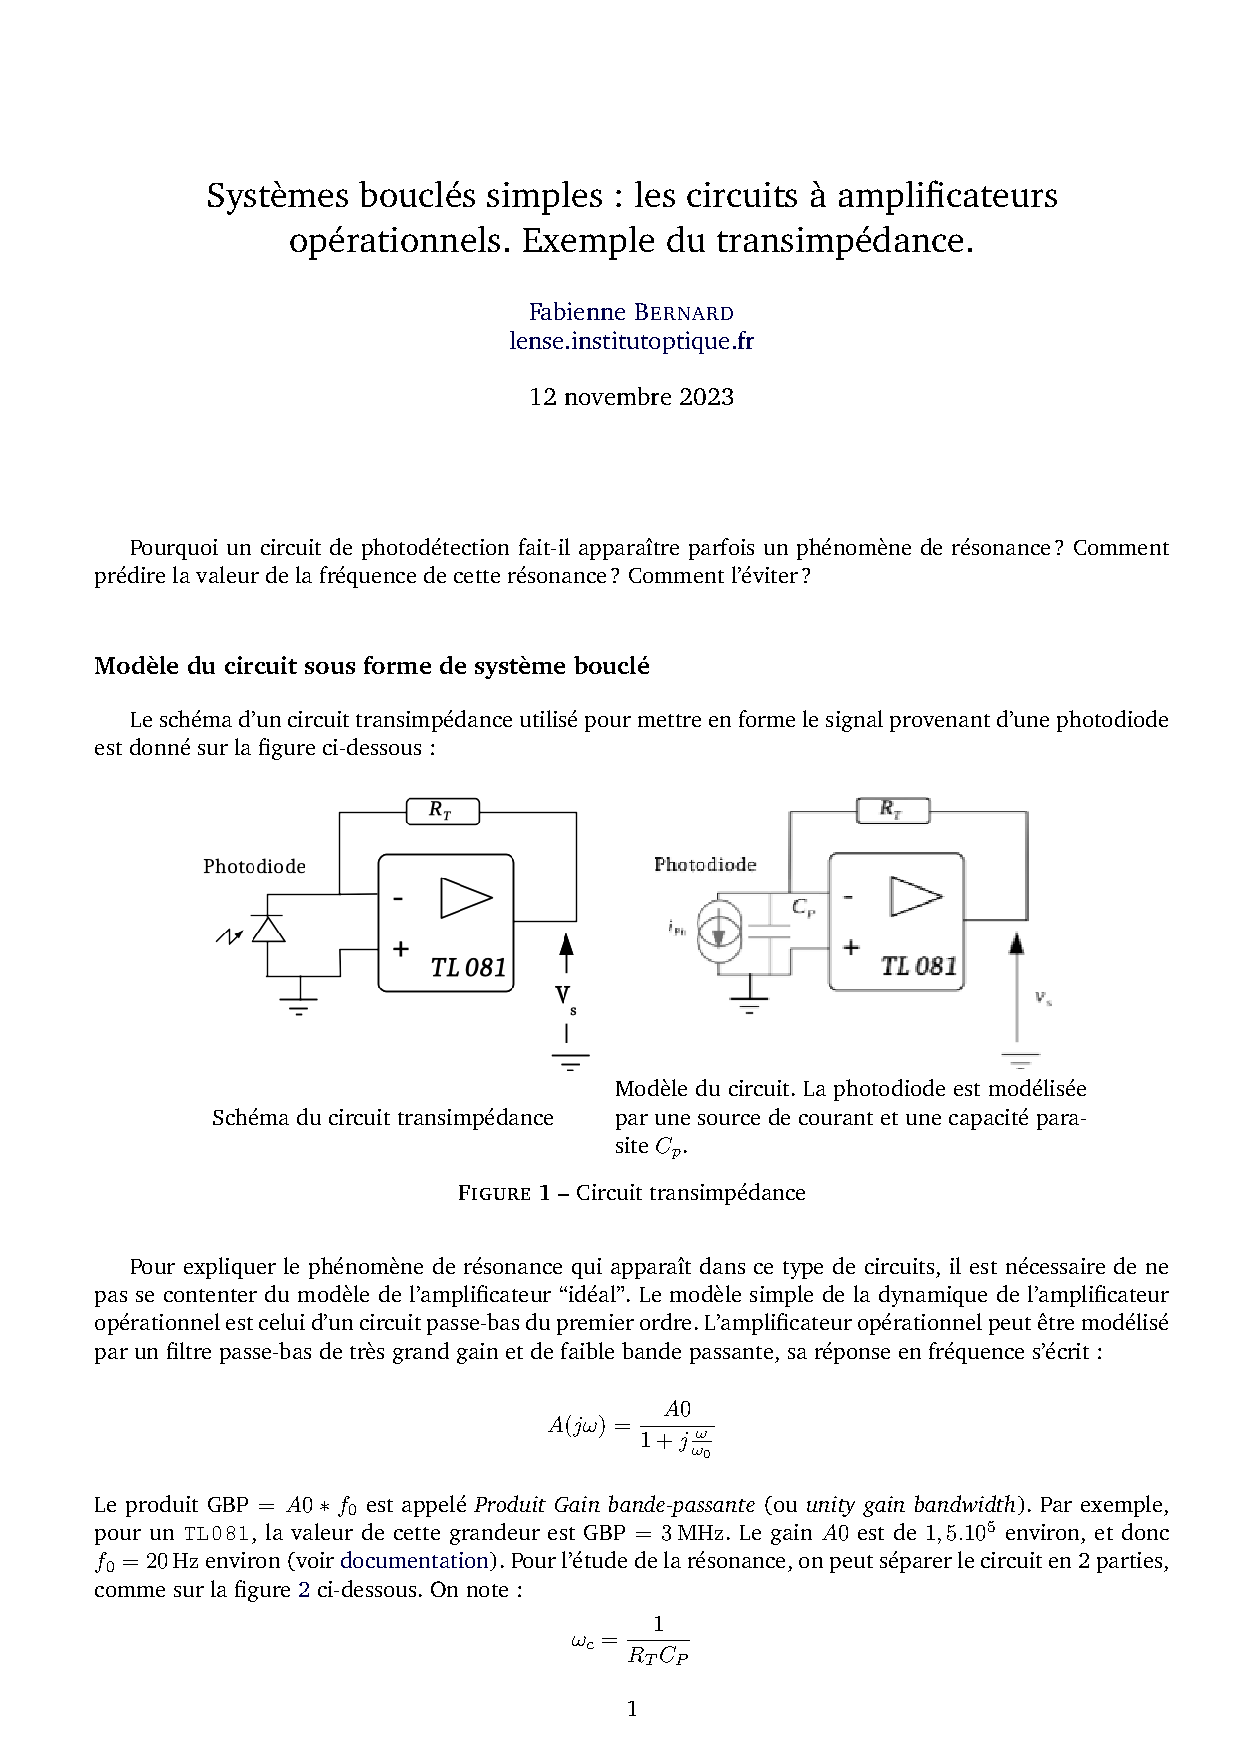
\includepdf[pages=1, pagecommand={\section{\texorpdfstring{\hspace{-1em}}{Annexe Transimpédance}}}\label{ressource:ModeleTrans}]{ressources/AnnexeTransImp.pdf}
\includepdf[pages=2-4]{ressources/AnnexeTransImp.pdf}

%% Fiches 
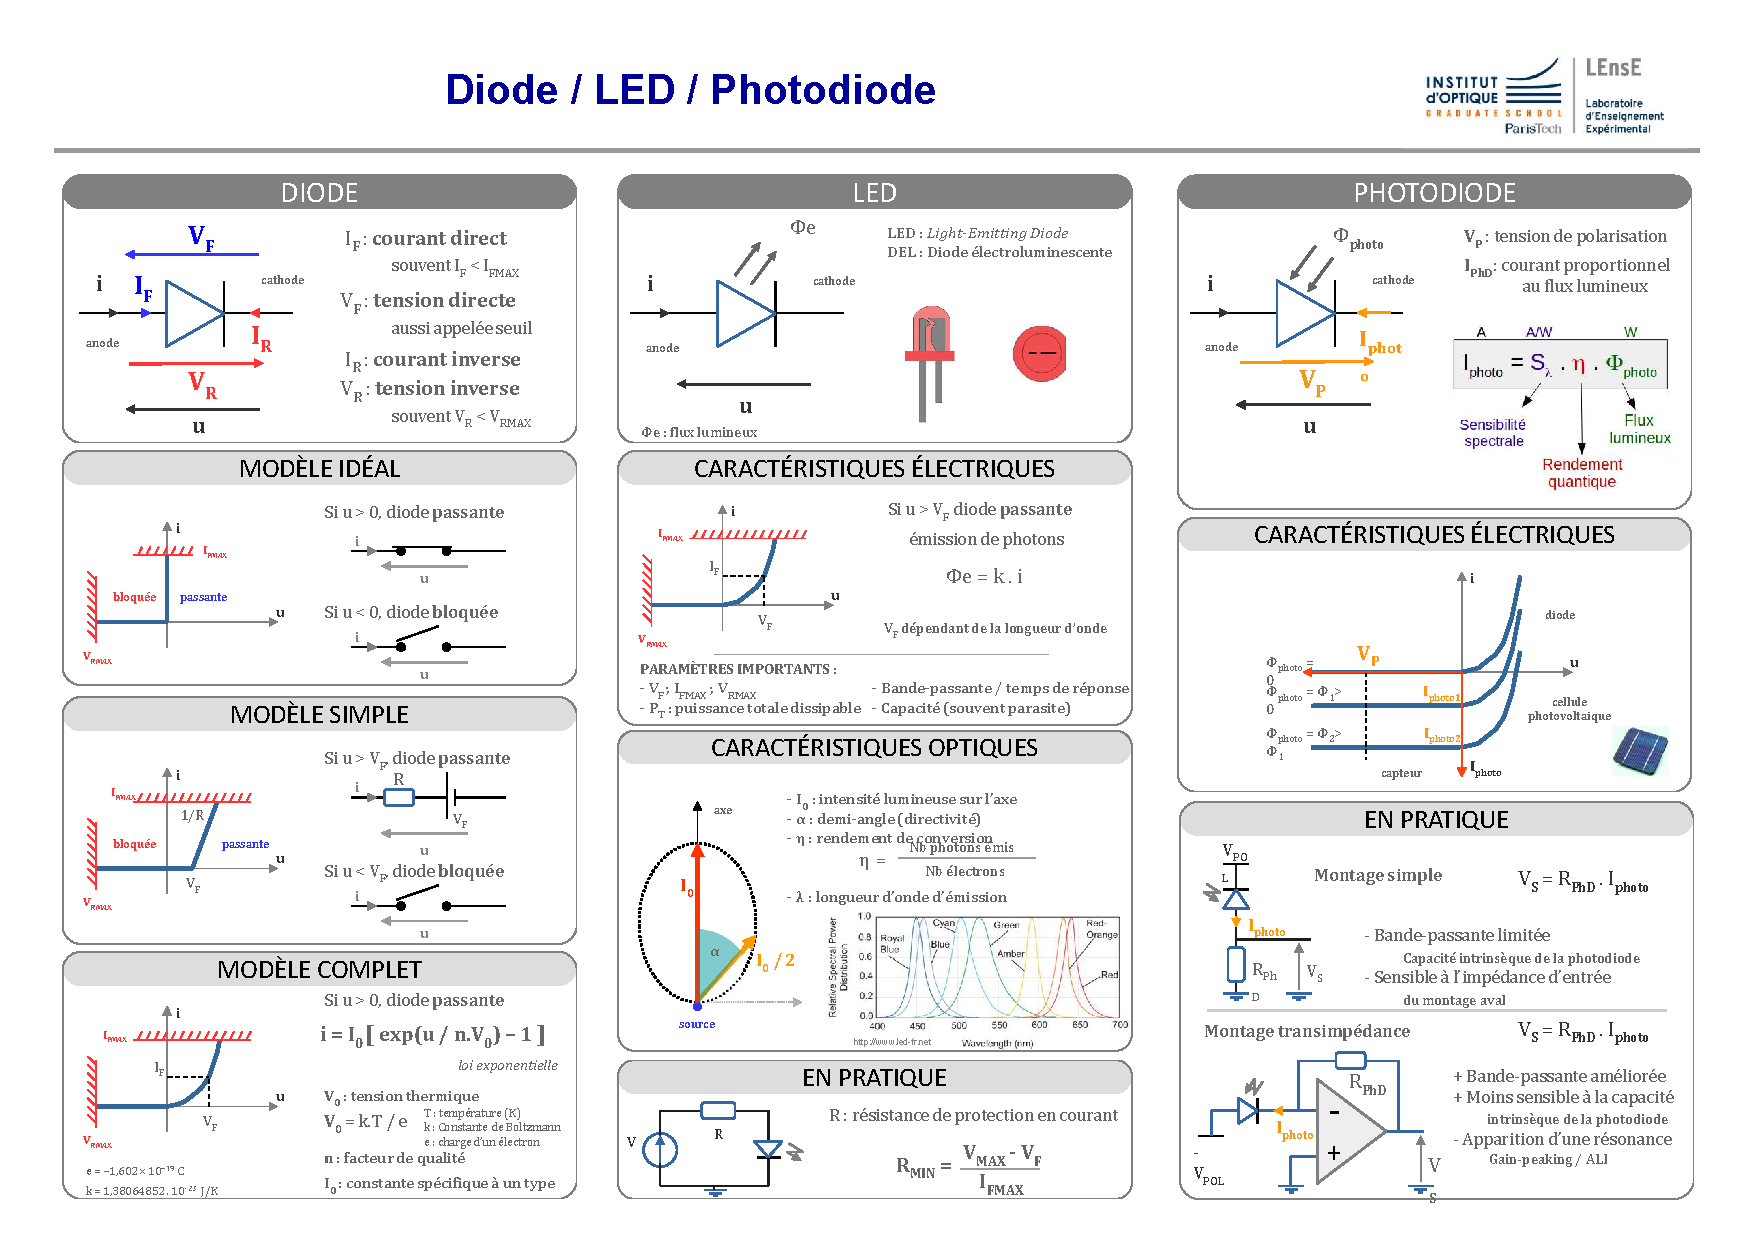
\includepdf[pages=-, landscape=true, pagecommand={\section{\texorpdfstring{\hspace{-1em}}{Fiche Diode / LED / Photodiode}}}\label{fiche:Led}]{../../Fiches/Fiche_Diode_LED_Photodiode.pdf}

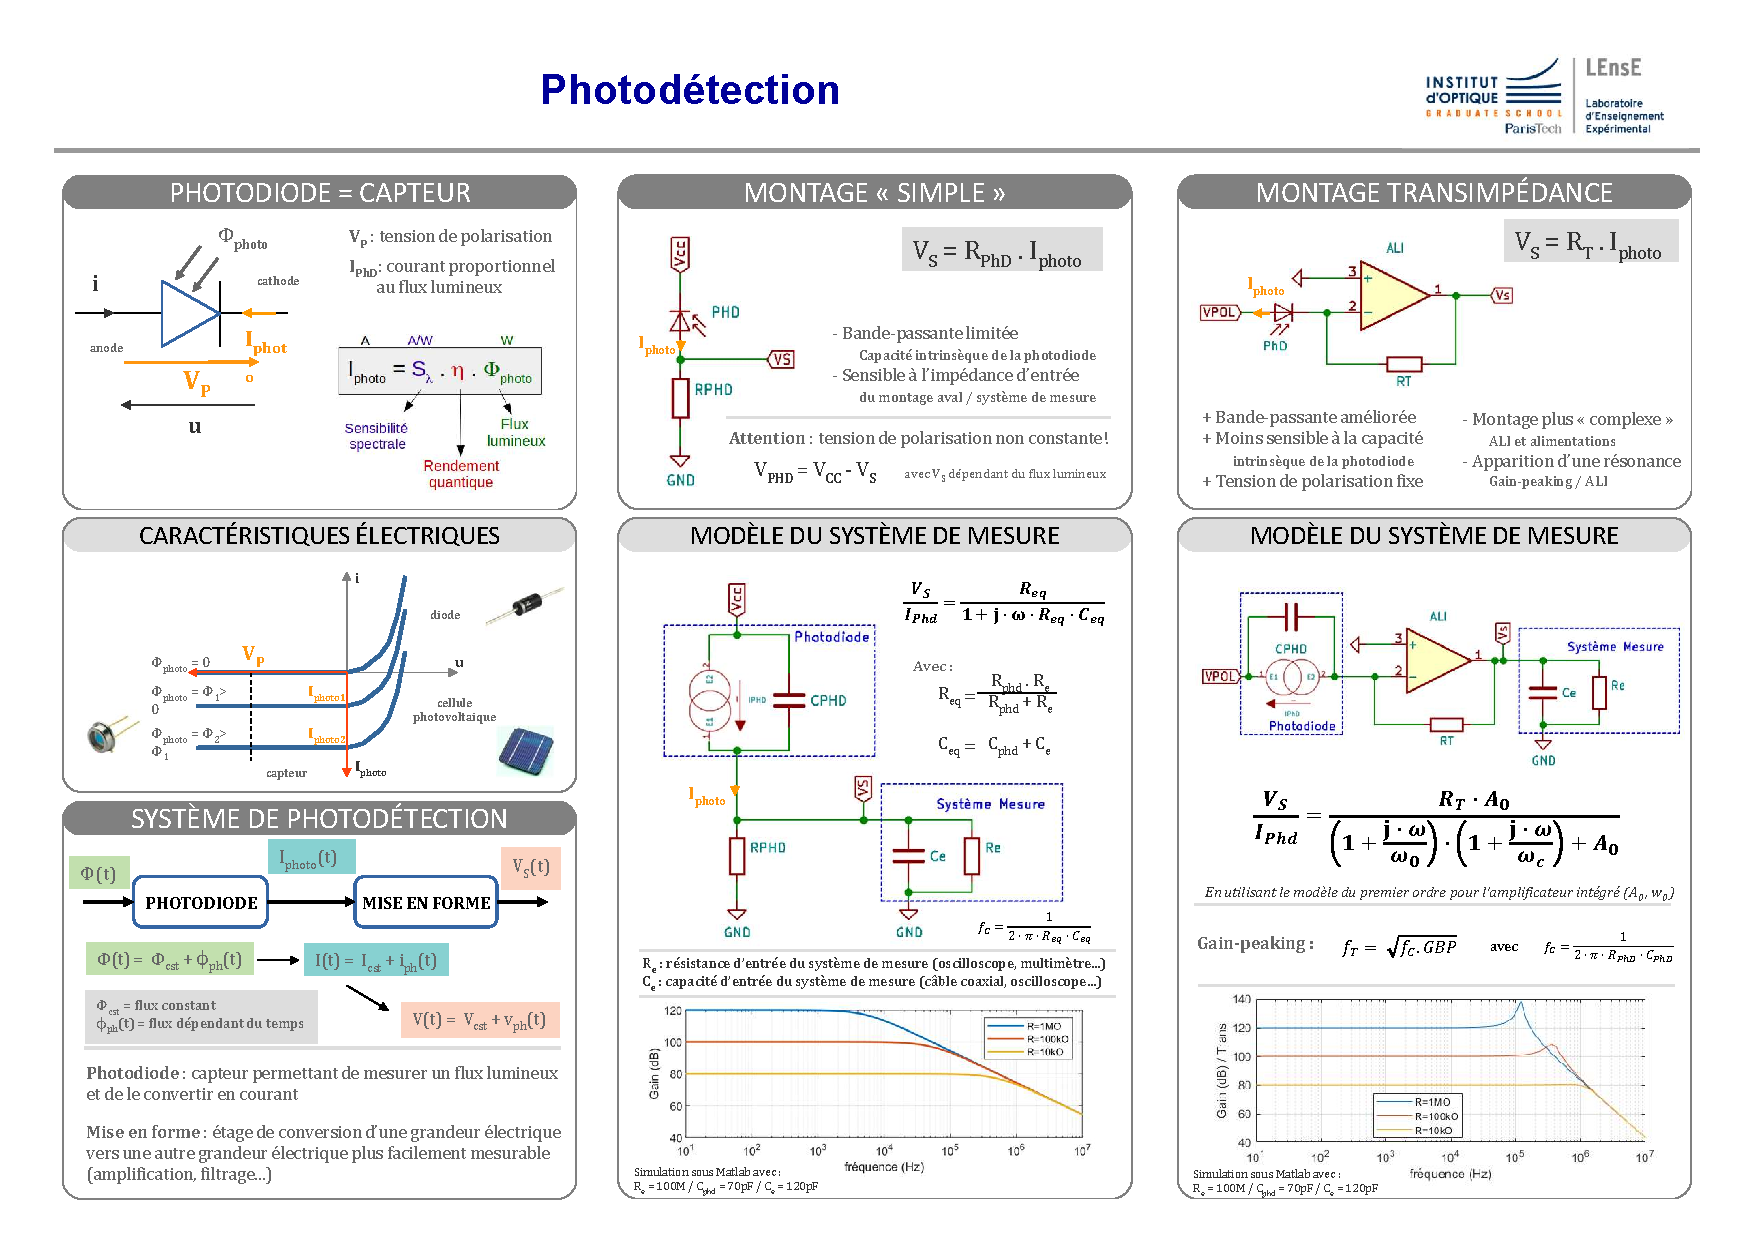
\includepdf[pages=-, landscape=true, pagecommand={\section{\texorpdfstring{\hspace{-1em}}{Fiche Photodétection}}}\label{fiche:Photodetect}]{../../Fiches/Fiche_Photodetection.pdf}

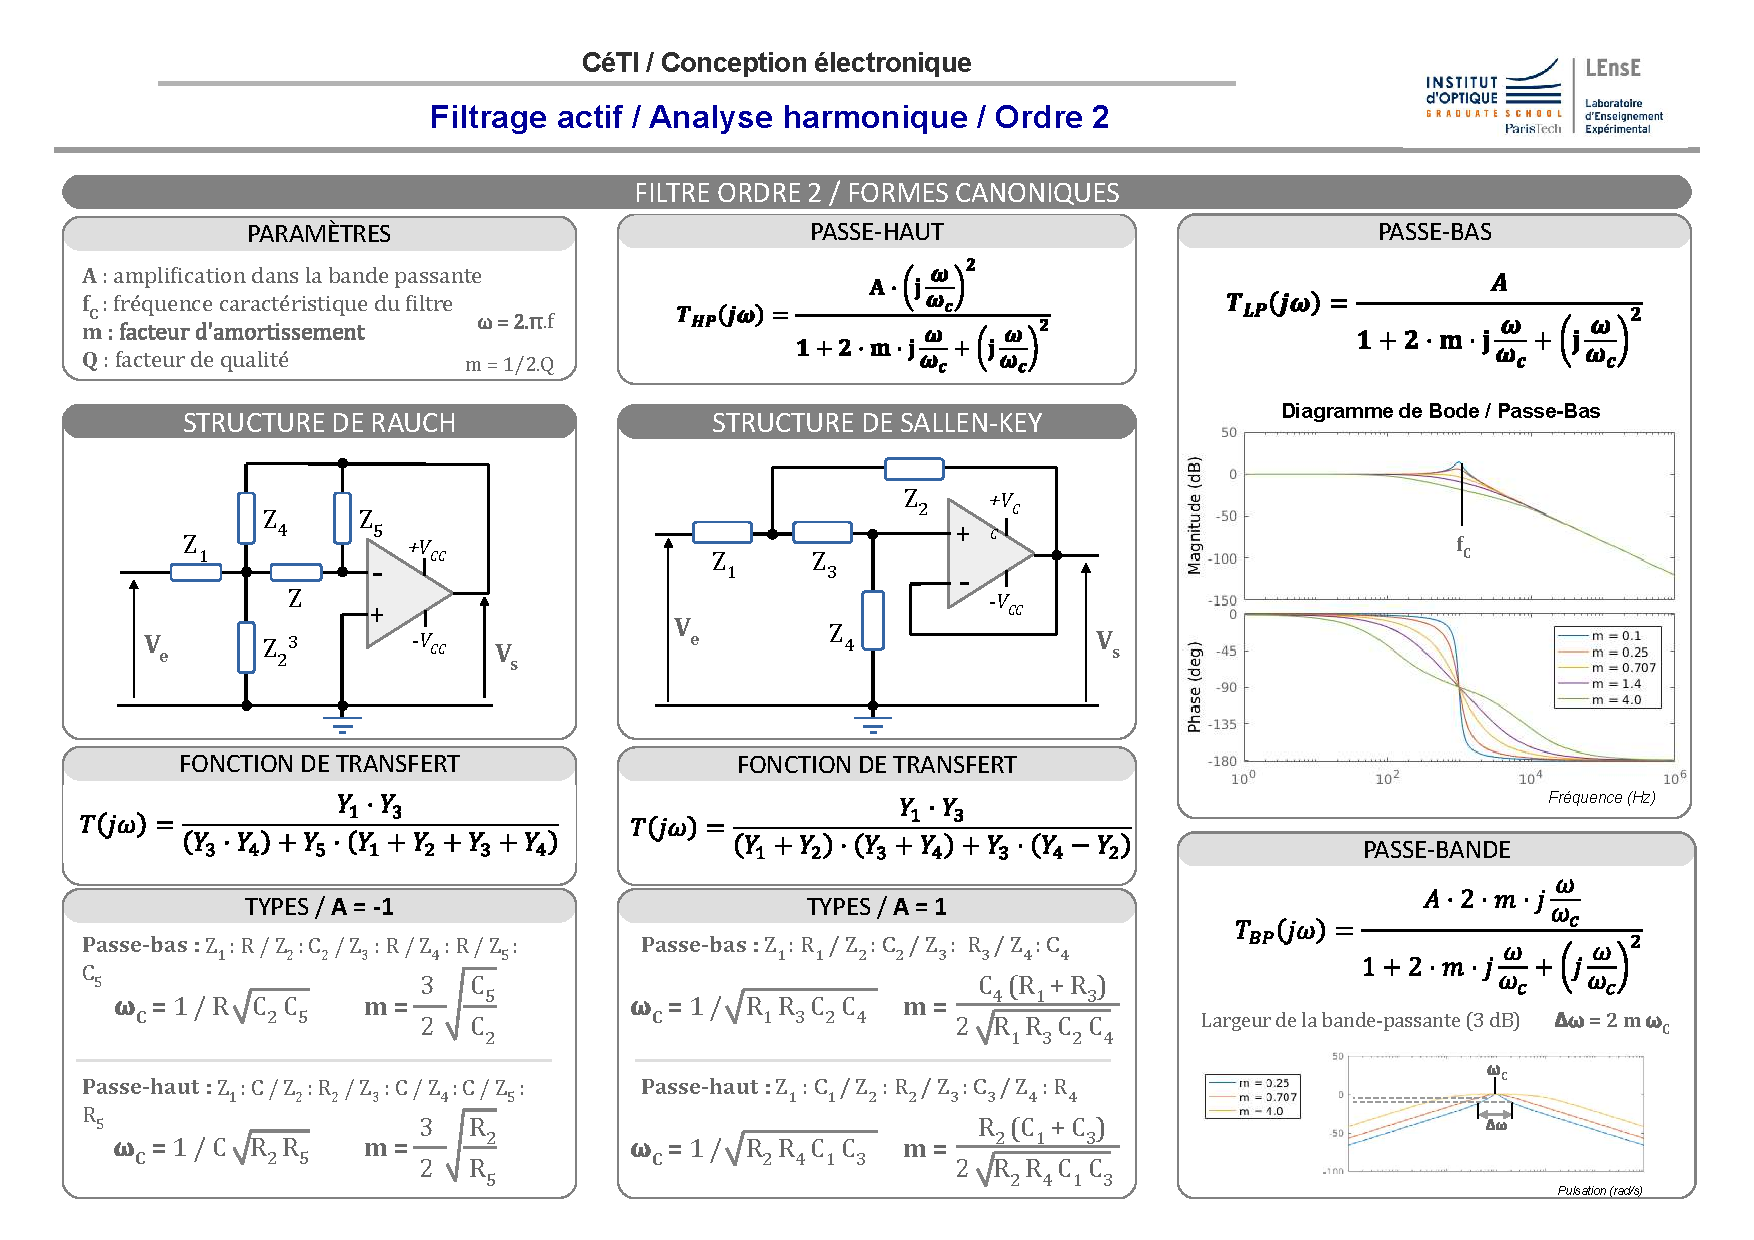
\includepdf[pages=-, landscape=true, pagecommand={\section{\texorpdfstring{\hspace{-1em}}{Fiche Analyse Harmonique Ordre 1}}}\label{fiche:AnHaOrdre2}]{../../Fiches/Fiche_Analyse_Ordre2.pdf}

\end{document}


